\newpage
\section{NOTA TEÓRICA}

Antes de iniciar con el uso y manipulación del lenguaje de programación C para la creación de los algoritmos objetivo del presente laboratorio, es necesario tener a mano una serie de conceptos importantes, los cuales se explican a continuación: 

\subsection{Microcontrolador ATtiny4313}
Tal como se detalla en la hoja del fabricante \cite{AT}, este componente corresponde a un microcontrolador de 8 bits, de alto rendimiento y de baja potencia, producido por la empresa Atmel. Cuenta con 120 instrucciones, una memoria flash con capacidad de 4 kb, una SRAM de 258 bytes y una memoria EEPROM de 258 bytes. Asimismo, cuenta con 18 GPIO programables, 2 timers (uno de 8 y otro de 16 bits), cuatro canales PWM, además de USI y una USART \textit{full duplex}. En la Figura \ref{fig:AT_pins} puede observarse la distribución de pines del microcontrolador y sus respectivas funciones:  

\begin{figure}[H]
\centering
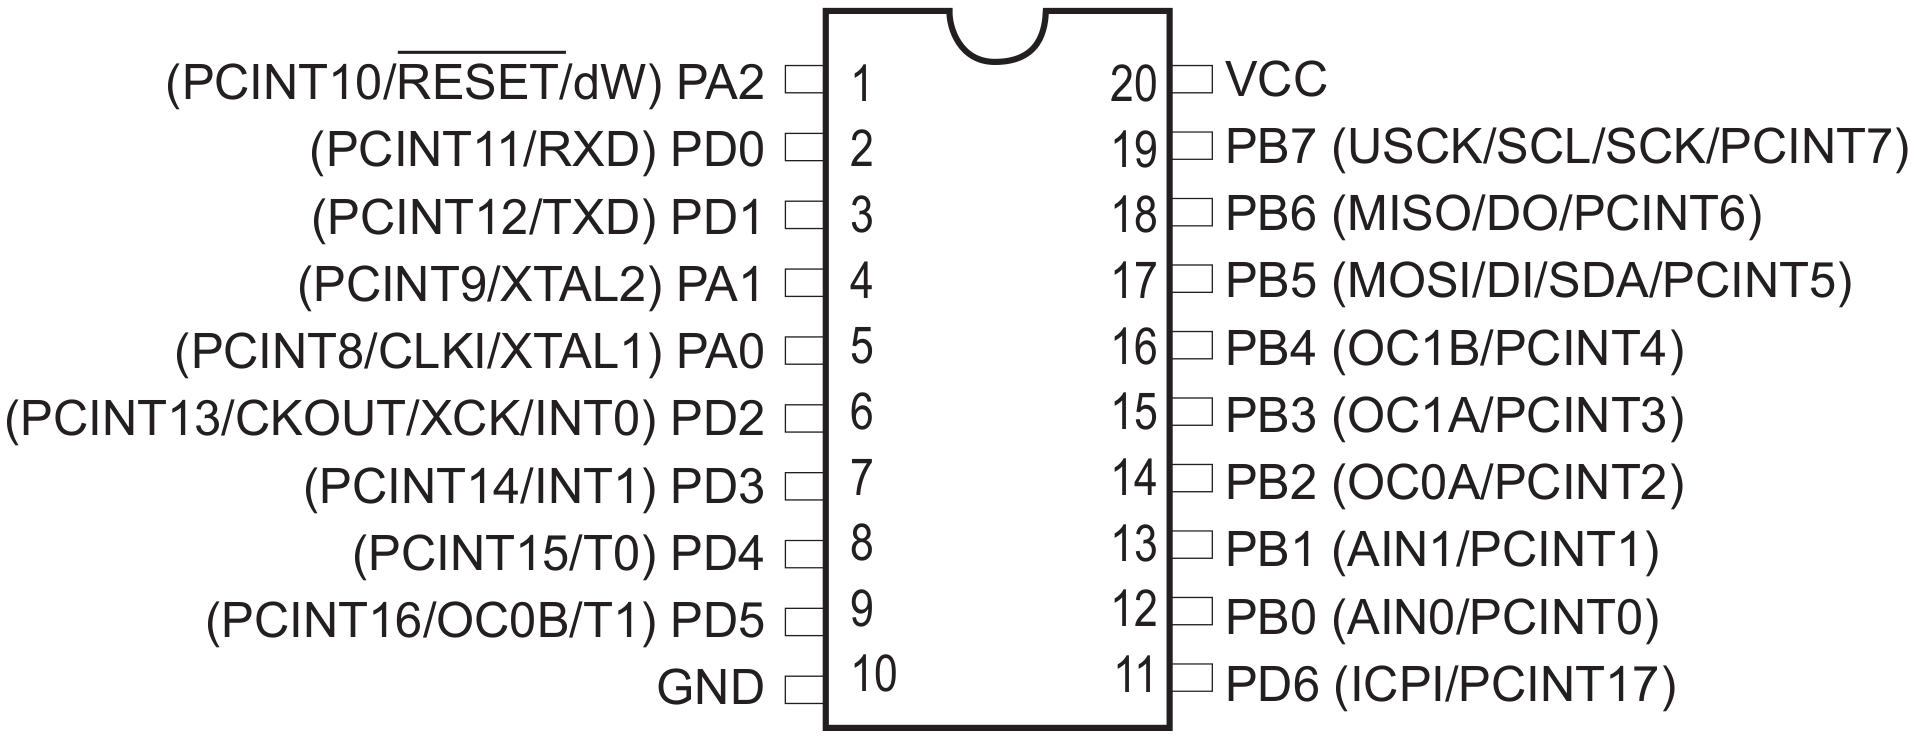
\includegraphics[width=140mm]{./Figuras/Nota_teorica/AT_pins}
\caption{Diagrama de pines y sus respectivas funciones. (Fuente: Imagen tomada de \cite{AT})}
\label{fig:AT_pins}
\end{figure}

Para el presente laboratorio, sólo serán de utilidad los pines que tienen la función de GPIO para la entrada y salida de información, además de las lineas de interrupción y temporización. Para más información general del dispositivo, observar el Anexo \ref{an:01_GEN}. Por otro lado, en la Figura \ref{fig:DBLO} puede consultarse el diagrama de bloques del microcontrolador en el cual puede consultarse a alto nivel la conexión interna de este (no incluye el CPU):

\begin{figure}[H]
\centering
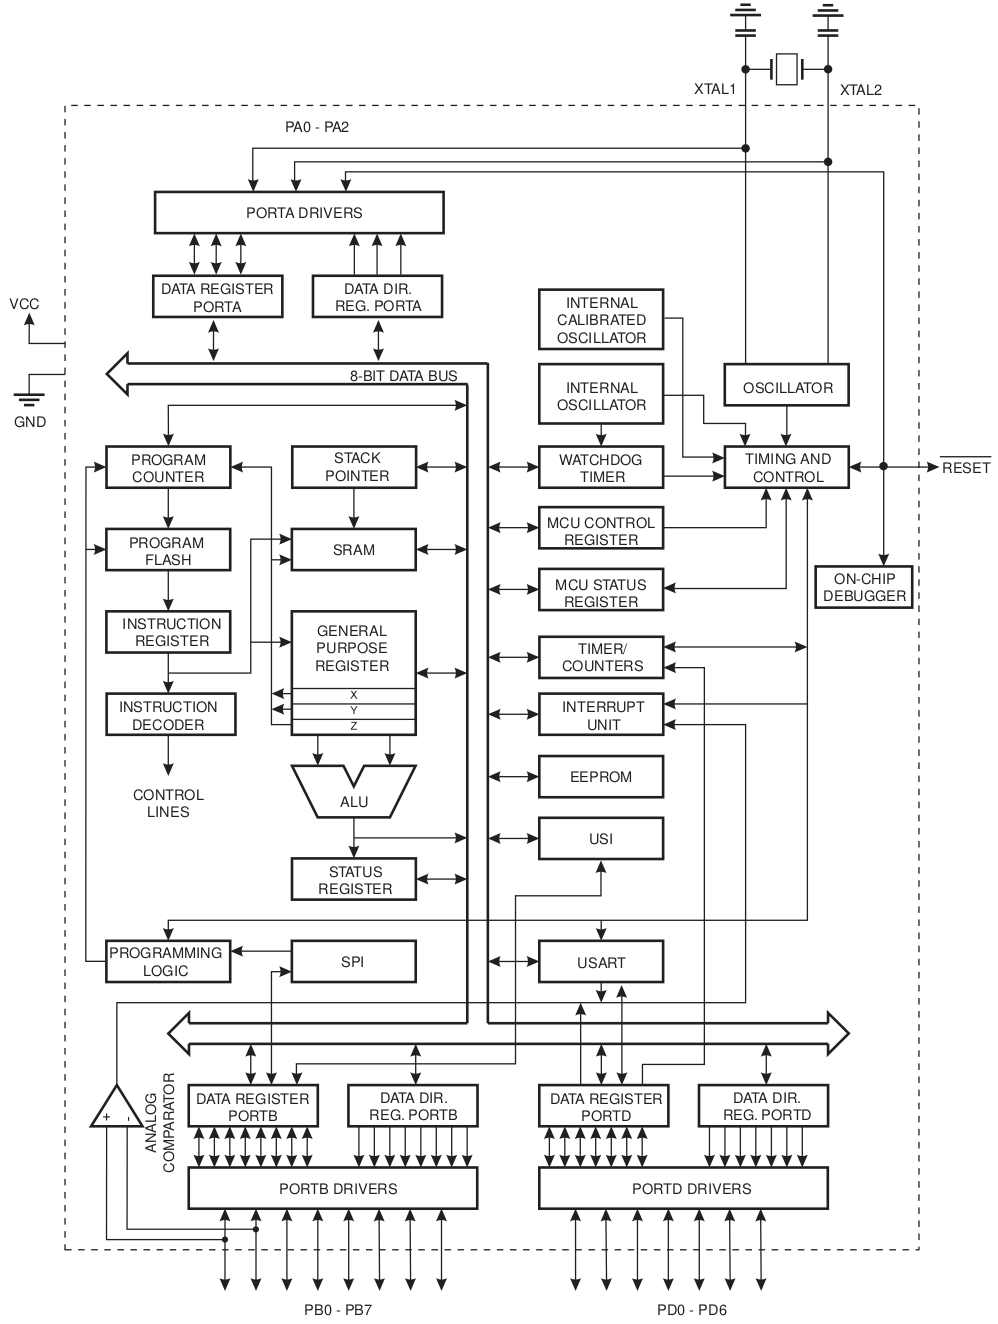
\includegraphics[width=160mm]{./Figuras/Nota_teorica/DBLO}
\caption{Diagrama de bloques del ATtiny4313. (Fuente: Imagen tomada de \cite{AT})}
\label{fig:DBLO}
\end{figure}

\subsubsection{Registros de importancia}
Para controlar la operación deseada del microcontrolador, es necesario colocar los valores adecuados en los distintos registros que contiene el dispositivo. Para el caso particular del presente laboratorio, los principales registros de interrupción se detallan a continuación, utilizando como base la hoja del fabricante \cite{AT}:

\begin{itemize}
    \item \textbf{DDRB - Port B Data Direction Register}: este registro permite configurar los pines del puerto B como entradas o salidas (si se define un pin en 1 es una salida, de lo contrario es un entrada). En la Figura \ref{fig:DDRB}, puede verse la composición del registro: 
  
    \begin{figure}[H]
    \centering
    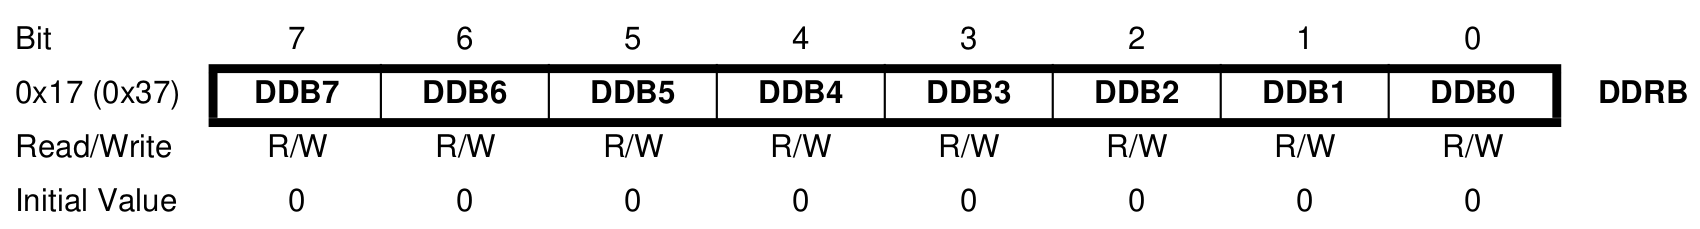
\includegraphics[width=150mm]{./Figuras/Nota_teorica/DDRB}
    \caption{Composición del \textit{Port B Data Direction Register}. (Fuente: Imagen tomada de \cite{AT})}
    \label{fig:DDRB}
    \end{figure}

    \item \textbf{PORTB - Port B Data Register}: corresponde a un puerto I/O bidireccional de 8 bits con resistencias de pull-up internas. Permiten determinar el estado de cada uno de los pines del puerto B. A continuación en la Figura \ref{fig:PORTB}, pueden observarse los detalles de configuración de este registro: 

    \begin{figure}[H]
    \centering
    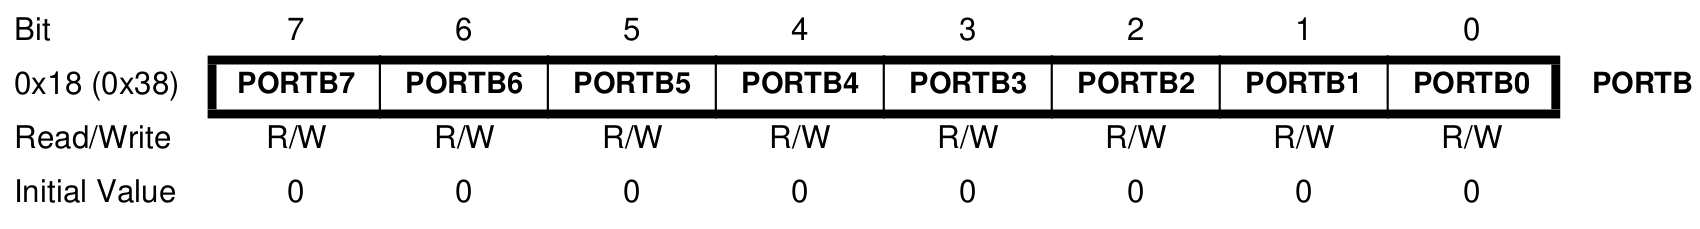
\includegraphics[width=150mm]{./Figuras/Nota_teorica/PORTB}
    \caption{Composición del \textit{Port B Data Register}. (Fuente: Imagen tomada de \cite{AT})}
    \label{fig:PORTB}
    \end{figure}
    
    \item \textbf{GIMSK -}: este permite habilitar o deshabilitar algunos tipos de interrupciones. Para el caso particular de este laboratorio, son importantes las interrupciones externas (INT0 e INT1). Los detalles del registro pueden verse en la Figura \ref{fig:GIMSK} a continuación: 

    \begin{figure}[H]
    \centering
    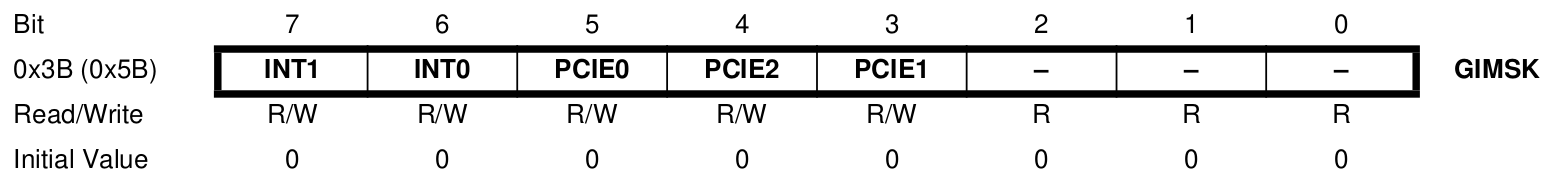
\includegraphics[width=150mm]{./Figuras/Nota_teorica/GIMSK}
    \caption{Composición del \textit{General Interrupt Mask Register}. (Fuente: Imagen tomada de \cite{AT})}
    \label{fig:GIMSK}
    \end{figure}
    
    \item \textbf{MCUCR - MCU Control Register}: este registro contiene bits de control que habilitan distintos modos de interpretar interrupciones. Su composición puede observarse en la Figura \ref{fig:MCUCR}

    \begin{figure}[H]
    \centering
    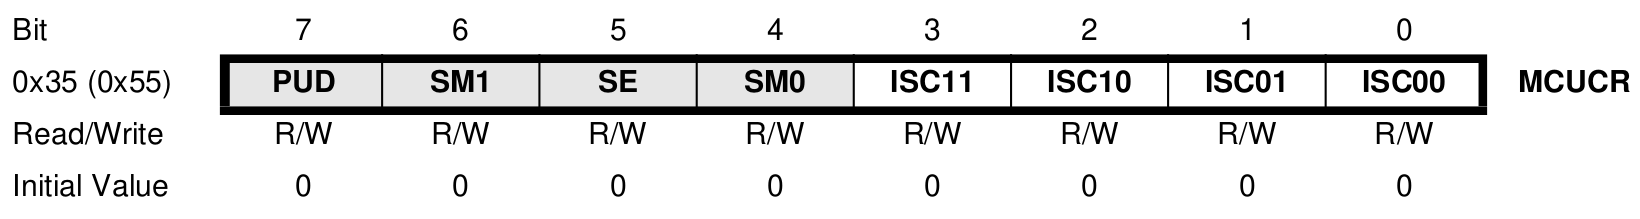
\includegraphics[width=150mm]{./Figuras/Nota_teorica/MCUCR}
    \caption{Composición del \textit{MCU Control Register}. (Fuente: Imagen tomada de \cite{AT})}
    \label{fig:MCUCR}
    \end{figure}

    En el caso de que la interrupción externa INT0 (del registro anterior) esté habilitada, este registro cuenta con distintas configuraciones, las cuales pueden observarse en la Tabla \ref{table:MCUCR}: 

    \begin{table}[!ht]
    \caption{Control de detección de interrupciones de INT0. (Tomada de \cite{AT}).}
    \begin{center}
    \begin{tabular}{c|c|c}
    \hline
    \textbf{ISC01}&\textbf{ISC00}&\textbf{Descripción}\\
    \hline
    0 & 0 & El nivel bajo de INT0 genera una petición de interrupción.\\\hline
    0 & 1 & Cualquier cambio lógico en INT0 genera una petición de interrupción.\\\hline
    1 & 0 & El flanco decreciente de INT0 genera una petición de interrupción.\\\hline
    1 & 1 & El flanco creciente de INT0 genera una petición de interrupción.\\
    \hline
    \end{tabular} \label{table:MCUCR}
    \end{center}
    \end{table}
\end{itemize}

Por otro lado, los principales registros de \textit{timing} (para el contador 0 - Timer0) para este laboratorio, pueden consultarse a continuación, utilizando como base la hoja del fabricante \cite{AT}:

\begin{itemize}
    \item \textbf{TCNT0 - Timer/Counter}: este registro da acceso directo al contador de 8 bits de la unidad \textit{Timer/Counter} y este acceso puede ser tanto de lectura como de escritura. En la Figura \ref{fig:TCNT0} puede verse su composición: 

    \begin{figure}[H]
    \centering
    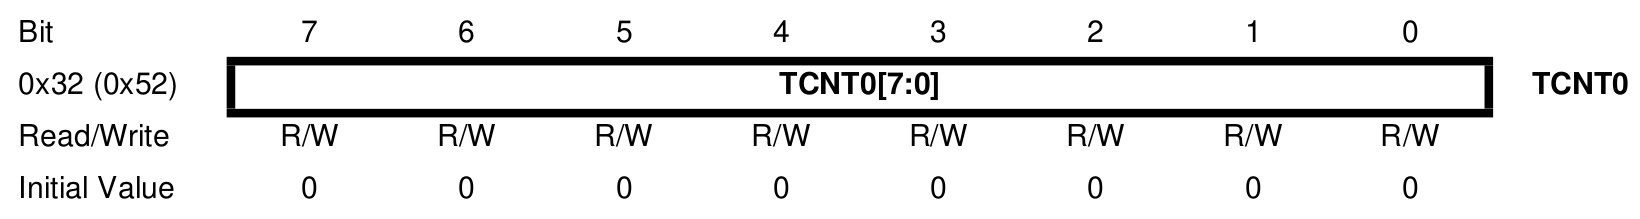
\includegraphics[width=150mm]{./Figuras/Nota_teorica/TCNT0}
    \caption{Composición del \textit{Timer/Counter}. (Fuente: Imagen tomada de \cite{AT})}
    \label{fig:TCNT0}
    \end{figure}

    \item \textbf{TCCR0A - Timer/Counter Control Register A}: este registro permite configurar la secuencia de conteo para el contador 0 y el modo de comparación. Su composición puede observarse en la Figura \ref{fig:TCCR0A}: 

    \begin{figure}[H]
    \centering
    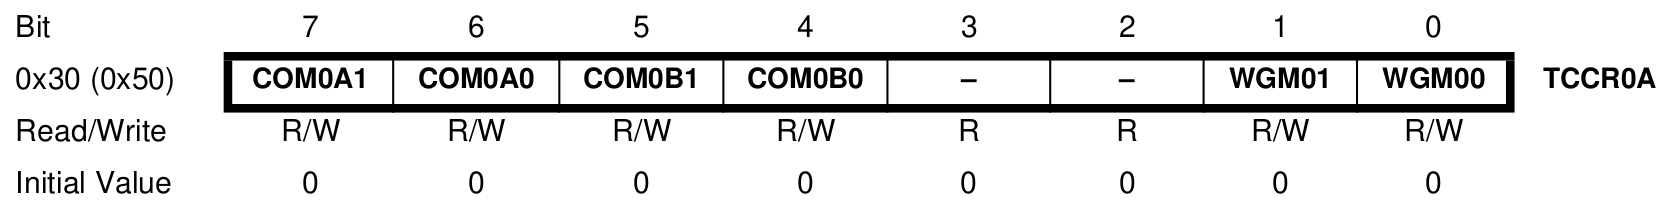
\includegraphics[width=150mm]{./Figuras/Nota_teorica/TCCR0A}
    \caption{Composición del \textit{Timer/Counter Control Register A}. (Fuente: Imagen tomada de \cite{AT})}
    \label{fig:TCCR0A}
    \end{figure}

    La secuencia de conteo es determinada por los bits WGM01 y WGM00, además del bit WGM02 de registro CCR0B (el siguiente). Los modos de comparación son determinados por combinaciones de los bits de secuencia de conteo y los birs COM0A1, COM0A0, COM0B1 y COM0B0. 

    
    \item \textbf{TCCR0B - Timer/Counter Control Register B}: este registro permite configurar la fuente de reloj, la cual es controlada por los bits CS02:0. Su composición puede observarse en la Figura \ref{fig:TCCR0B}: 
    
    \begin{figure}[H]
    \centering
    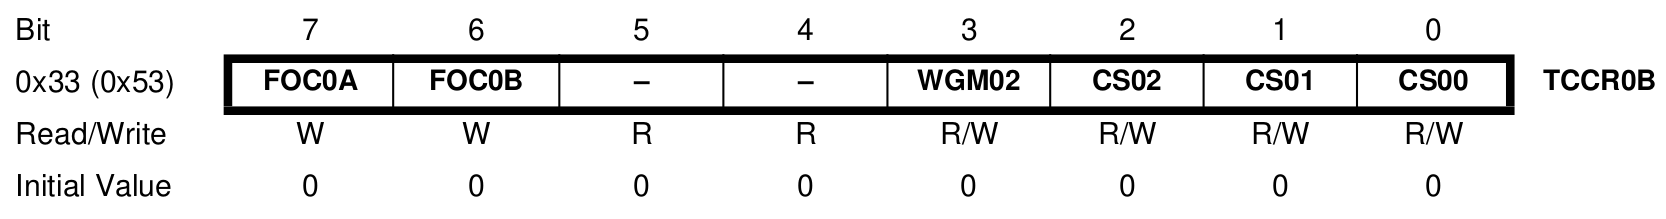
\includegraphics[width=150mm]{./Figuras/Nota_teorica/TCCR0B}
    \caption{Composición del \textit{Timer/Counter Control Register B}. (Fuente: Imagen tomada de \cite{AT})}
    \label{fig:TCCR0B}
    \end{figure}

    La distintas configuraciones posibles pueden observarse en la Tabla \ref{table:TCCR0B}:

    \begin{table}[!ht]
    \caption{Descripción de los bits de selección de reloj. (Tomada de \cite{AT}).}
    \begin{center}
    \begin{tabular}{c|c|c|l}
    \hline
    \textbf{CS02}&\textbf{CS01}&\textbf{CS00}&\textbf{Descripción}\\
    \hline
    0 & 0 & 0 & Sin fuente de reloj (Timer/Counter detenido).\\\hline
    0 & 0 & 1 & $clk_{I/O}$ / (Sin \textit{prescaling}).\\\hline
    0 & 1 & 0 & $clk_{I/O}$ / 8 (Del \textit{prescaler}).\\\hline
    0 & 1 & 1 & $clk_{I/O}$ / 64 (Del \textit{prescaler}).\\\hline
    1 & 0 & 0 & $clk_{I/O}$ / 256 (Del \textit{prescaler}).\\\hline
    1 & 0 & 1 & $clk_{I/O}$ / 1024 (Del \textit{prescaler}).\\\hline
    1 & 1 & 0 & Fuente de reloj externa en el pin T0. Reloj en flanco decreciente.\\\hline
    1 & 1 & 1 & Fuente de reloj externa en el pin T0. Reloj en flanco creciente.\\\hline
    \end{tabular} \label{table:TCCR0B}
    \end{center}
    \end{table}
    
    \item \textbf{TIMSK - Timer/Counter Interrupt Mask Register}: este registro permite la selección del tipo de interrupciones causadas por el contador 0 (\textit{Timer/Counter Compare Match} A y B, además de interrupción por \textit{overflow}). Los detalles del registro pueden verse en la Figura \ref{fig:TIMSK}: 

    \begin{figure}[H]
    \centering
    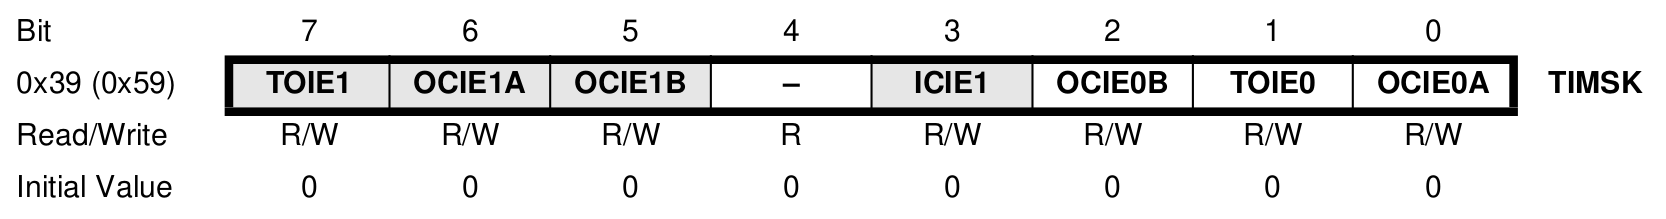
\includegraphics[width=150mm]{./Figuras/Nota_teorica/TIMSK}
    \caption{Composición del \textit{Timer/Counter Interrupt Mask Register}. (Fuente: Imagen tomada de \cite{AT})}
    \label{fig:TIMSK}
    \end{figure}
\end{itemize}

\subsection{Resistencia de \textit{pull-down}}\label{sec:cir0}
Del enunciado del laboratorio, se sabe que el objetivo de este es construir un simulador de un paso peatonal que cuente con dos botones de entrada con los que el usuario pueda solicitar una parada del tránsito vehicular. De lo anterior se puede deducir que al menos uno de los pines del microcontrolador debe ser configurado como entrada y que esta debe permanecer en un estado determinado, para que sólo en caso de presionar el botón (se obtiene el inverso del estado anterior), se active su funcionamiento. Para ese diseño, se quiere que el estado por defecto sea en bajo para proteger el circuito constantemente y que el estado en alto (al presionar el botón) active el circuito. 

Una resistencia de pull-down permite lograr el comportamiento deseado para el caso expuesto. En la Figura \ref{fig:pullD} puede observarse la disposición adecuada construida en SimulIDE según se detalla en \cite{pullU}: 

\begin{figure}[H]
\centering
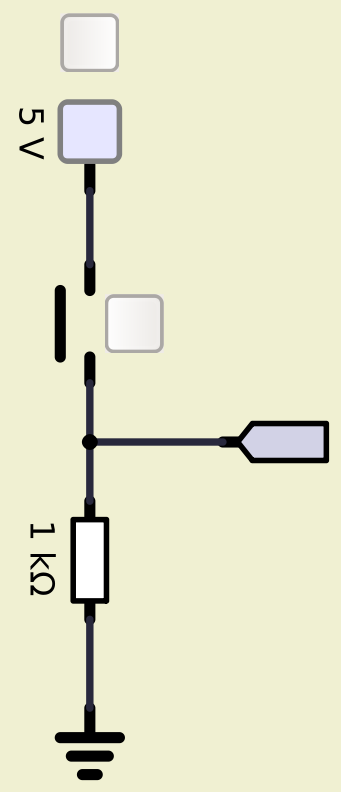
\includegraphics[width=40mm]{./Figuras/Nota_teorica/pullD}
\caption{Ejemplo de resistencia de \textit{pull-down} y \textit{switch} en SimulIDE.}
\label{fig:pullD}
\end{figure}

En la Figura \ref{fig:pullD}, puede observarse como el pulsador está conectado entre la fuente de tensión y el pin del MCU. Cuando el interruptor es presionado, la entrada del microcontrolador está en un valor lógico alto, pero cuando el interruptor está abierto, la resistencia \textit{pull-down} ``jala'' la tensión de entrada a la tierra (valor lógico cero). Según se explica en \cite{pullU}, la resistencia \textit{pull-down} debe ser mayor que la impedancia de salida del dispositivo, ya que de lo contrario podría ser capaz de bajar la tensión demasiado y la tensión de entrada en el pin se mantendría en un valor bajo lógico constante. Para calcular esta, se aplica la ley de Ohm de la siguiente forma: 

\begin{equation}
    Z_{MCU} = \frac{V_{DD}}{I_{max}}
\end{equation}

Donde $V_{DD}$ corresponde a la tensión máxima entregada por cada pin del MCU y $I_{max}$ la corriente máxima en el mismo caso, de esta forma se tiene que: 

\begin{equation}
    Z_{MCU} = \frac{5}{20 \times 10^{-3}} = 250 \; \Omega
\end{equation}

Para este caso particular, se tomará su valor como 1 k$\Omega$ para asegurarse de que no haya ningún problema.

\subsection{Circuito para lidiar con el \textit{switch bounce}} \label{sec:cir1}
Tal como se detalla en \cite{RC}, cerrar un \textit{switch}, puede parecer que este hace contacto de manera absoluta e inmediata, sin embargo, este dispositivo no deja de ser mecánico y el contacto ocurre de manera oscilante, por lo que una serie de interferencias son ingresadas a la señal transmitida. Para solucionar este problema, puede utilizarse un circuito RC a la salida del interruptor, de tal forma que se filtren los picos producidos por las oscilaciones y suavicen la señal que será transmitida. Lo anterior es útil para evitar falsas pulsaciones. Un ejemplo del tipo de circuito a construir es el que puede observarse en la Figura \ref{fig:RC1}: 

\begin{figure}[H]
\centering
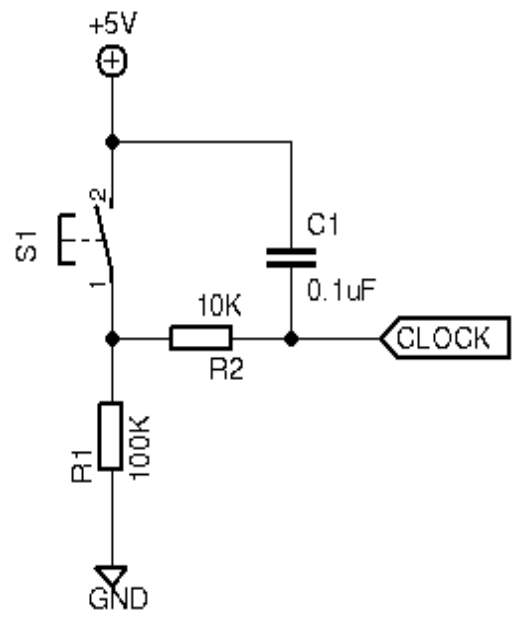
\includegraphics[width=80mm]{./Figuras/Nota_teorica/RC1}
\caption{Ejemplo de circuito utilizado para evitar las oscilaciones producidas por un \textit{switch} que combina un circuito RC con un resistor de \textit{pull-down}. (Fuente: Imagen tomada de \cite{RC})}
\label{fig:RC1}
\end{figure}

Para hacer los cálculos adecuados de capacitancia y resistencia, se inicia definiendo un tiempo de carga y descarga adecuado. En este caso, como no se trata de una acción que necesite de actividad inmediata, se puede trabajar en el orden de los milisegundos, en este caso, de los 100 ms. Como bien se sabe: 

\begin{equation}
    \tau = R \cdot C
\end{equation}

Por lo que si ya se tiene un valor de tiempo, basta con seleccionar una de las dos variables restantes para despejar la otra. Si se toma un valor de resistencia de 5 k$\Omega$, entonces despejando:

\begin{equation}
    C = \frac{\tau}{R} = \frac{10 \times 10^{-3}}{5 \times 10^{3}} = 2 \; \mu F
\end{equation}

\noindent Para apegarse a los valores disponibles en el mercado, se elige un capacitor de 2.2 $\mu$F. 

El circuito resultante construido en SimulIDE puede consultarse en la Figura \ref{fig:RC2} a continuación: 

\begin{figure}[H]
\centering
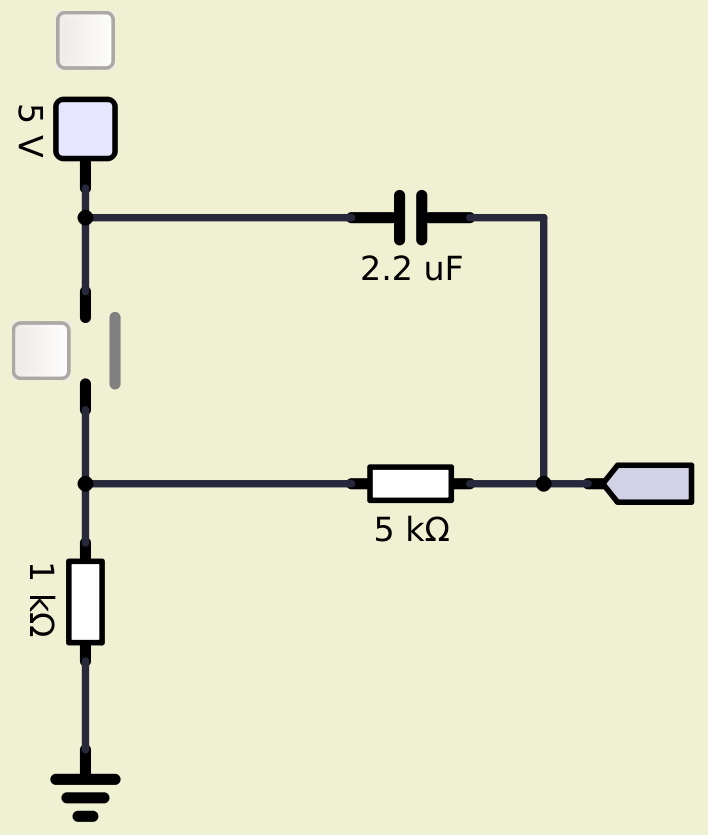
\includegraphics[width=70mm]{./Figuras/Nota_teorica/RC2}
\caption{Circuito utilizado para evitar las oscilaciones producidas por un \textit{switch} que combina un circuito RC con un resistor de \textit{pull-down}.}
\label{fig:RC2}
\end{figure}

Del enunciado se sabe que para simular un paso peatonal, serán necesarios dos botones, uno para cada semáforo peatonal. A pesar de ser botones distintos, la funcionalidad que activan (interrupción externa en INT0 que modifica la FSM) en la misma, por lo que deben colocarse en paralelo. El circuito resultante construido en SimulIDE puede consultarse en la Figura \ref{fig:RC3} a continuación: 

\begin{figure}[H]
\centering
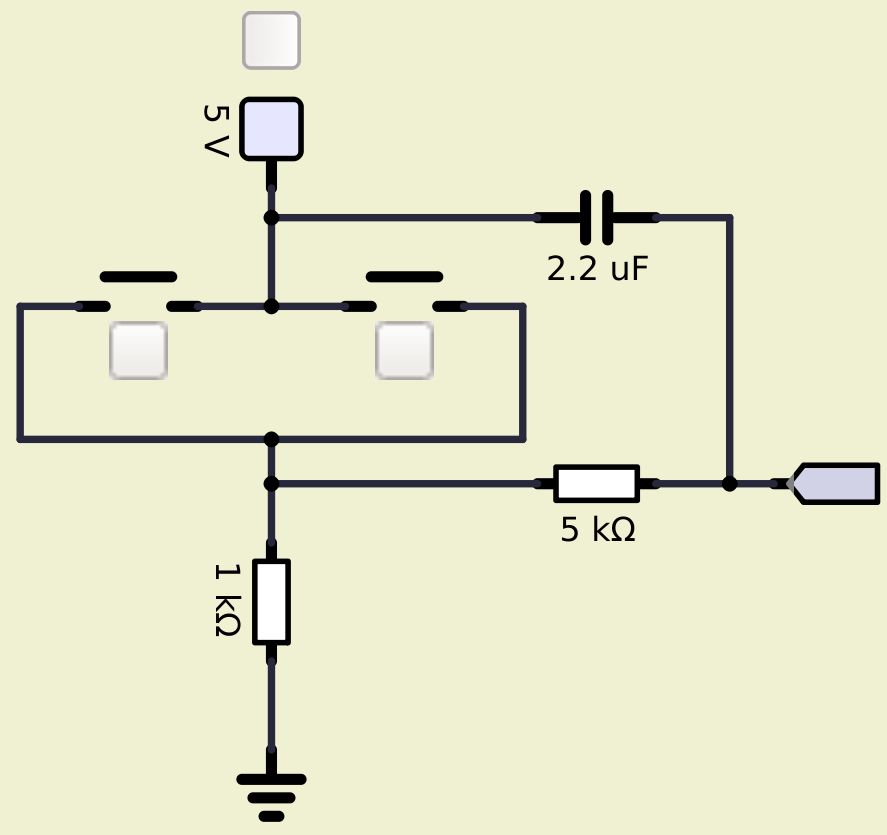
\includegraphics[width=100mm]{./Figuras/Nota_teorica/RC3}
\caption{Circuito utilizado para evitar las oscilaciones producidas por dos \textit{switches} que combina un circuito RC con un resistor de \textit{pull-down}.}
\label{fig:RC3}
\end{figure}

\subsection{Diseño del circuito simulador de un paso peatonal} \label{sec:cir2}
Según se indica en el enunciado, el presente laboratorio tiene como objetivo simular el funcionamiento de un paso peatonal de una calle unidireccional que cuenta con dos semáforos peatonales y un semáforo vehicular. La Figura \ref{fig:enun} muestra la disposición de los elementos mencionados: 

\begin{figure}[H]
\centering
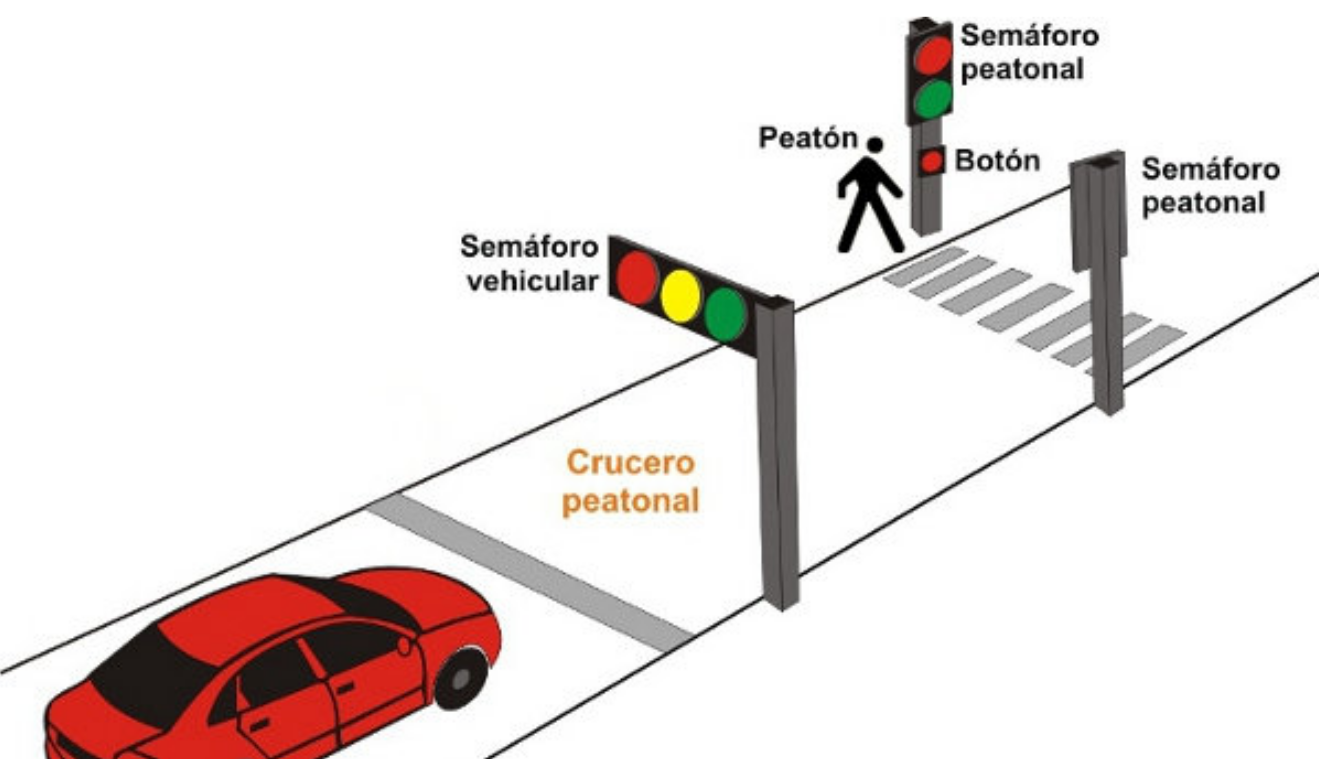
\includegraphics[width=120mm]{./Figuras/Nota_teorica/enun}
\caption{Cruce peatonal.}
\label{fig:enun}
\end{figure}

De la Figura \ref{fig:enun}, se puede deducir que habrán 7 LEDs conectados entre alguno de los pines del ATtiny4313 y la tierra, por lo que estos necesitan de resistencias de protección. Para calcular el valor de estas, se debe tomar en cuenta que la tensión máxima de operación es de 5 V y la corriente máxima suministrada es de 20 mA, información tomada de la hoja del fabricante \cite{AT}. Para obtener el valor de la resistencia de protección utilizando la ley de Kirchhoff de esta forma:

\begin{equation}
    R = \frac{V_{DD} - V_{LED}}{I_{max}} 
\end{equation}

Como se trata de una simulación, se tomará $V_{LED}$ = 2.4 V (tensión de umbral del simulador) para todos los casos. Para no presionar el sistema, se realizarán los cálculos utilizando 15 mA. De esta forma: 

\begin{equation}
    R = \frac{5 - 2.4}{15 \times 10^{-3}} = 173.33 \; \Omega
\end{equation}

\noindent Es este caso, se selecciona un valor estándar de 180 $\Omega$. 

\subsection{Lista de componentes y precios}

En la Tabla \ref{table:Equipo} pueden consultarse los componentes utilizados y sus precios, tomando como referencia los precios del sitio web de la tienda de componentes MicroJPM (\url{https://www.microjpm.com/}): 

\begin{table}[H]
\caption{Lista de componentes.}
\begin{center}
\begin{tabular}{c|c|c}
\hline
\textbf{Componente}&\textbf{Cantidad}&\textbf{Precio}\\
\hline
ATtiny4313 & 1 & \$1,80\\
Pulsador & 2 & \$0,40\\
Capacitor de 2.2 $\mu$F & 1 & \$0,35\\
Resistor de 5 k$\Omega$ & 1 & \$0,07\\
Resistor de 1 k$\Omega$ & 1 & \$0,07\\
Resistores de 180 $\Omega$ & 7 & \$0,35\\
LED verdes & 3 & \$0.51\\ 
LED rojos & 3 & \$0.51\\ 
LED amarillo & 1 & \$0,17\\ 
\hline
Total & - & \$4.23\\
\end{tabular} \label{table:Equipo}
\end{center}
\end{table}

Según la Tabla \ref{table:Equipo}, para realizar este proyecto son necesario ₡2,121.73, según el valor del dólar al momento de escribir el presente informe. 


\subsection{Máquinas de estado finitas (FSM)}

Una Maquina de estado Finito es esencialmente un programa que representa una secuencia de instrucciones a ser ejecutadas, donde cada instrucción depende del estado actual de la máquina y del actual estimulo. Las posibles entradas al sistema son una secuencia de símbolos seleccionadas desde un conjunto finito l de símbolos de entrada, y las salidas resultantes son secuencias de símbolos escogidas desde un conjunto finito Z de símbolos de salida \cite{alavi2016maquinas}. 
Estas maquinas pueden ser síncronas o asíncronas, cuando necesitan o no la intervención de un pulso de reloj.
Existen dos tipos principales de maquinas de estado:
\begin{itemize}
    \item \textbf{Maquina de estado de Mealy}: Las salidas de la máquina de estados no solo dependen de los estados, sino también de las entradas al sistema, que se representan definiendo salidas de la máquina en las transiciones \cite{Maquinadeestados}.
    \item \textbf{Maquina de estado de Moore}: Las salidas de la máquina de estados solo dependen del estado del sistema, que se representa definiendo salidas de la máquina en los estados, según se detalla en \cite{Maquinadeestados}. 
\end{itemize}

En la Figura \ref{fig:FSMej} puede consultarse un ejemplo de máquina de estado: 

\begin{figure}[H]
\centering
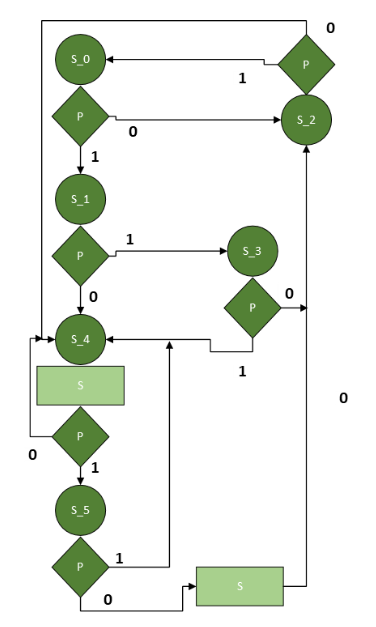
\includegraphics[scale=1.1]{./Figuras/Nota_teorica/Diagrama_de_stados_viejo}
\caption{Diagrama FSM ejemplo (Elaboración propia).}
\label{fig:FSMej}
\end{figure}